\documentclass[12pt]{article}

% Автор стиля: Сергей Копелиович
% Автор конспекта: Игорь Смирнов 

\usepackage{cmap}
\usepackage[T2A]{fontenc}
\usepackage[utf8]{inputenc}
\usepackage[russian]{babel}
\usepackage{graphicx}
\usepackage{amsthm,amsmath,amssymb}
\usepackage{listings}
\usepackage{color}
\usepackage{xcolor}
\usepackage[normalem]{ulem}
\usepackage{array}
\usepackage{epigraph}

\usepackage[russian,colorlinks=true,urlcolor=red,linkcolor=blue]{hyperref}
\usepackage{enumerate}
\usepackage{datetime}
\usepackage{fancyhdr}
\usepackage{lastpage}
\usepackage{verbatim}
\usepackage{tikz}
\usetikzlibrary{arrows,decorations.markings,decorations.pathmorphing}
\usepackage{pgfplots}

\usepackage{ifthen}
\usepackage{mathtools}

%\usepackage{tabls}
%\usepackage{tabularx}
%\usepackage{xifthen}
%\listfiles

\def\SEASON{Технологии компьютерных сетей}

\input code-format.tex

\sloppy
\voffset=-20mm
\textheight=235mm
\hoffset=-22mm
\textwidth=180mm
\headsep=12pt
\footskip=20pt

\parskip=0em
\parindent=0em

\setlength\epigraphwidth{.8\textwidth}

\newlength{\tmplen}
\newlength{\tmpwidth}
\newcounter{listcounter}

% Список с маленькими отступами
\newenvironment{MyList}[1][4pt]{
  \begin{enumerate}[1.]
  \setlength{\parskip}{0pt}
  \setlength{\itemsep}{#1}
}{       
  \end{enumerate}
}
% Вложенный список с маленькими отступами
\newenvironment{InnerMyList}[1][0pt]{
  \vspace*{-0.5em}
  \begin{enumerate}[(a)]
  \setlength{\parskip}{-0pt}
  \setlength{\itemsep}{#1}
}{       
  \end{enumerate}
  \vspace*{-0.5em}
}
% Список с маленькими отступами
\newenvironment{MyItemize}[1][4pt]{
  \begin{itemize}
  \setlength{\parskip}{0pt}
  \setlength{\itemsep}{#1}
}{       
  \end{itemize}
}

% Основные математические символы
\def\TODO{{\color{red}\bf TODO}}
\def\N{\mathbb{N}}       %
\def\R{\mathbb{R}}       %
\def\F2{\mathbb{F}_2}    %
\def\Z{\mathbb{Z}}       %
\def\INF{\t{+}\infty}    % +inf
\def\EPS{\varepsilon}    %
\def\EMPTY{\varnothing}  %
\def\PHI{\varphi}        %
\def\SO{\Rightarrow}     % =>
\def\EQ{\Leftrightarrow} % <=>
\def\t{\texttt}          % mono font
\def\c#1{{\rm\sc{#1}}}   % font for classes NP, SAT, etc
\def\O{\mathcal{O}}      %
\def\NO{\t{\#}}          % #
\def\XOR{\text{ {\raisebox{-2pt}{\ensuremath{\Hat{}}}} }}
\renewcommand{\le}{\leqslant}
\renewcommand{\ge}{\geqslant}
\newcommand{\q}[1]{\langle #1 \rangle}               % <x>
\newcommand\URL[1]{{\footnotesize{\url{#1}}}}        %
% \newcommand{\sfrac}[2]{{\scriptscriptstyle\frac{#1}{#2}}}  % Очень маленькая дробь
% \newcommand{\mfrac}[2]{{\scriptstyle\frac{#1}{#2}}}    % Небольшая дробь
\newcommand{\sfrac}[2]{{\scriptstyle\frac{#1}{#2}}}  % Очень маленькая дробь
\newcommand{\mfrac}[2]{{\textstyle\frac{#1}{#2}}}    % Небольшая дробь

\newcommand{\fix}[1]{{\color{fixcolor}{#1}}} % \underline
\def\bonus{\t{\red{(*)}}}
\def\ifbonus#1{\ifthenelse{\equal{#1}{}}{}{\bonus}}
\def\smallsquare{$\scalebox{0.5}{$\square$}$}

\newlength{\myItemLength}
\setlength{\myItemLength}{0.3em}
\def\ItemSymbol{\smallsquare}
\def\Item{\vspace*{\myItemLength}\ItemSymbol \ \ }

\newcommand{\LET}{%
  % [line width=0.6pt]
  \begin{tikzpicture}%
  \draw(0.8ex,0) -- (0.8ex,1.6ex);%
  \draw(0,1.6ex) -- (0.8ex,1.6ex);%
  \end{tikzpicture}%
  \hspace*{0.1em}%
}

% Отступы
\def\makeparindent{\hspace*{\parindent}\unskip}
\def\up{\vspace*{-0.5em}}%{\vspace*{-\baselineskip}}
\def\down{\vspace*{0.5em}}
\def\LINE{\vspace*{-1em}\noindent \underline{\hbox to 1\textwidth{{ } \hfil{ } \hfil{ } }}}
\def\BOX#1{\mbox{\fbox{\bf{#1}}}}
\def\Pagebreak{\pagebreak\vspace*{-1.5em}}

% Мелкий заголовок
\newcommand{\THEE}[1]{
  \vspace*{0.5em}
  \noindent{\bf \underline{#1}}%\hspace{0.5em}
  \vspace*{0.2em}
}
% Другой тип мелкого заголовка
\newcommand{\THE}[1]{
  \vspace*{0.5em} $\bullet$
  \noindent{\bf #1}%\hspace{0.5em}
  \vspace*{0.2em}
}

\newenvironment{MyTabbing}{
  \t\bgroup
  \vspace*{-\baselineskip}
  \begin{tabbing}
    aaaa\=aaaa\=aaaa\=aaaa\=aaaa\=aaaa\kill
}{
  \end{tabbing}
  \t\egroup
}

% Код с правильными отступами
\lstnewenvironment{code}{
  \lstset{}
%  \vspace*{-0.2em}
}%
{
%  \vspace*{-0.2em}
}
\lstnewenvironment{codep}{
  \lstset{language=python}
}%
{
}

% Формулы с правильными отступами
\newenvironment{smallformula}{
 
  \vspace*{-0.8em}
}{
  \vspace*{-1.2em}
  
}
\newenvironment{formula}{
 
  \vspace*{-0.4em}
}{
  \vspace*{-0.6em}
  
}

% Большая квадратная скобка
\makeatletter
\newenvironment{sqcases}{%
  \matrix@check\sqcases\env@sqcases
}{%
  \endarray\right.%
}
\def\env@sqcases{%
  \let\@ifnextchar\new@ifnextchar
  \left\lbrack
  \def\arraystretch{1.2}%
  \array{@{}l@{\quad}l@{}}%
}
\makeatother

% Определяем основные секции: \begin{Lm}, \begin{Thm}, \begin{Def}, \begin{Rem}
\renewcommand{\qedsymbol}{$\blacksquare$}
\theoremstyle{definition} % жирный заголовок, плоский текст
\newtheorem{Thm}{\underline{Теорема}}[subsection] % нумерация будет "<номер subsection>.<номер теоремы>"
\newtheorem{Lm}[Thm]{\underline{Lm}} % Нумерация такая же, как и у теорем
\newtheorem{Ex}[Thm]{Упражнение} % Нумерация такая же, как и у теорем
\newtheorem{Example}[Thm]{Пример} % Нумерация такая же, как и у теорем
\newtheorem{Code}[Thm]{Код} % Нумерация такая же, как и у теорем
\theoremstyle{plain} % жирный заголовок, курсивный текст
\newtheorem{Def}[Thm]{Def} % Нумерация такая же, как и у теорем
\theoremstyle{remark} % курсивный заголовок, плоский текст
\newtheorem{Cons}[Thm]{Следствие} % Нумерация такая же, как и у теорем
\newtheorem{Conj}[Thm]{Гипотеза} % Нумерация такая же, как и у теорем
\newtheorem{Prop}[Thm]{Утверждение} % Нумерация такая же, как и у теорем
\newtheorem{Rem}[Thm]{Замечание} % Нумерация такая же, как и у теорем
\newtheorem{Remark}[Thm]{Замечание} % Нумерация такая же, как и у теорем
\newtheorem{Algo}[Thm]{Алгоритм} % Нумерация такая же, как и у теорем

% Определяем ЗАГОЛОВКИ
\def\SectionName{unknown}
\def\AuthorName{unknown}

\newlength{\sectionvskip}
\setlength{\sectionvskip}{0.5em}
\newcommand{\Section}[4][]{
  % Заголовок
  \pagebreak
%  \ifthenelse{\isempty{#1}}{
    \refstepcounter{section}
%  }{}
  \vspace{0.5em}
%  \ifthenelse{\isempty{#1}}{
%    \addtocontents{toc}{\protect\addvspace{-5pt}}%
    \addcontentsline{toc}{section}{\arabic{section}. #2}
%  }{}
  \begin{center}
    {\Large \bf Тема \NO{\arabic{section}}: #2} \\ 
    \vspace{\sectionvskip}
    {\large #3} \\
  \end{center}

  \LINE

  % Запомнили название и автора главы
  \gdef\SectionName{#2}
  \gdef\AuthorName{#4}

  % Заголовок страницы
  %\lhead{Алгоритмы, \SEASON}
  \chead{}
  \rhead{\SectionName}
  \renewcommand{\headrulewidth}{0.4pt}

  \lfoot{Глава \NO{\arabic{section}}. #3.}
  \cfoot{\thepage\t{/}\pageref*{LastPage}}
  \rfoot{Автор конспекта: \AuthorName}
  \renewcommand{\footrulewidth}{0.4pt}
}

\newcommand{\Subsection}[2][]{
  \refstepcounter{subsection}
  \vspace*{1em}
  \ifthenelse{\equal{#1}{}}
    {\addcontentsline{toc}{subsection}{\arabic{section}.\arabic{subsection}. #2}}
    {\addcontentsline{toc}{subsection}{\arabic{section}.\arabic{subsection}. \bonus\,#2}}
  {\color{blue}\bf\large \arabic{section}.\arabic{subsection}. \ifbonus{#1}\,{#2}} 
  \vspace*{0.5em}
  \makeparindent
}
\newcommand{\Subsubsection}[2][]{
  \refstepcounter{subsubsection}
  \vspace*{1em}
  \ifthenelse{\equal{#1}{}}
    {\addcontentsline{toc}{subsubsection}{\arabic{section}.\arabic{subsection}.\arabic{subsubsection}. #2}}
    {\addcontentsline{toc}{subsubsection}{\arabic{section}.\arabic{subsection}.\arabic{subsubsection}. \bonus\,#2}}
  {\color{blue}\bf\large \arabic{section}.\arabic{subsection}.\arabic{subsubsection}. \ifbonus{#1}\,#2}
  \vspace*{0.5em}
  \makeparindent
}

\newcommand{\Header}{
  \pagestyle{empty}
  \renewcommand{\dateseparator}{--}
  \begin{center}
    {\Large\bf 
     НИУ ВШЭ СПб, \SEASON\\
    \vspace{0.3em}
     Конспект лекций}\\
    \vspace{0.7em}
    {Собрано {\today} в {\currenttime}}
  \end{center}

  \LINE
  \vspace{0em}

  \renewcommand{\baselinestretch}{0.98}\normalsize
  \tableofcontents
  \renewcommand{\baselinestretch}{1.0}\normalsize
  \pagebreak
}

\newcommand{\BeginConspect}{
  \pagestyle{fancy}
  \setcounter{page}{1}
}

\definecolor{mygray}{rgb}{0.7,0.7,0.7}
\definecolor{ltgray}{rgb}{0.9,0.9,0.9}
\definecolor{fixcolor}{rgb}{0.7,0,0}
\definecolor{red2}{rgb}{0.7,0,0}
\definecolor{dkred}{rgb}{0.4,0,0}
\definecolor{dkblue}{rgb}{0,0,0.6}
\definecolor{dkgreen}{rgb}{0,0.6,0}
\definecolor{brown}{rgb}{0.5,0.5,0}

\newcommand{\green}[1]{{\color{green}{#1}}}
\newcommand{\black}[1]{{\color{black}{#1}}}
\newcommand{\red}[1]{{\color{red}{#1}}}
\newcommand{\dkred}[1]{{\color{dkred}{#1}}}
\newcommand{\blue}[1]{{\color{blue}{#1}}}
\newcommand{\dkgreen}[1]{{\color{dkgreen}{#1}}}

\begin{document}

\Header

\BeginConspect

\Section{Архитектуры компьютерных сетей}{Лекция 1}{Игорь Смирнов}

\Subsection{Эталонная модель ISO/OSI}

Компьютерные сети существуют давно (с 50-60 годов прошлого века), а потом появилось миллион протоколов и люди поняли, что невозможно связывать между собой различные системы. Тогда организация ISO создала стандарт OSI~--- эталонная модель взаимодействия открытых систем. Задачи поделены на 7 уровней. Для каждого уровня описаны функции и элементы данных, которыми компьютеры обмениваются на этом уровне.

\begin{figure}[H]
  \centering
  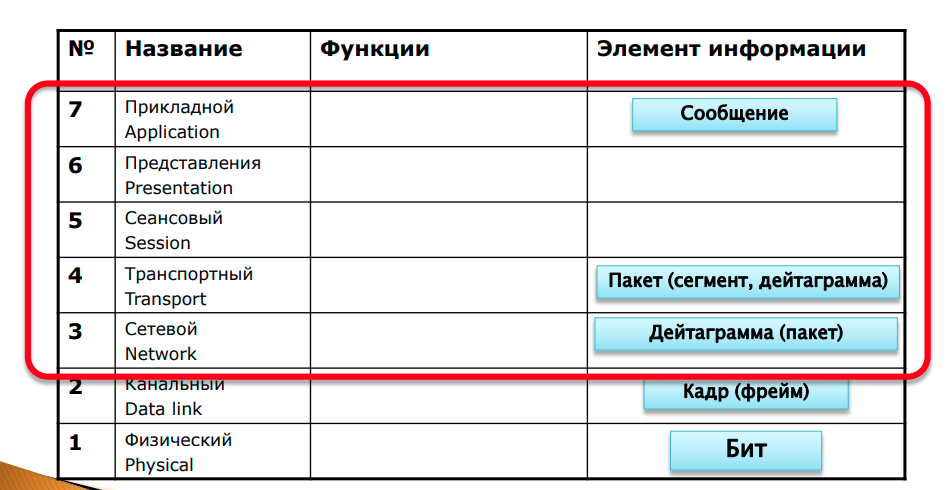
\includegraphics[width=15cm]{images/00/01}
\end{figure}

Иногда под физическим уровнем рисуют физическую среду, а над прикладным приложение/пользователя.

Эта стандартизация позволяет сравнивать между собой разные архитектуры и понимать, что за протокол используется и какая у него функциональная нагрузка.

\begin{enumerate}

\item Физический уровень позволяет соединить между собой два устройства и передать минимальную единицу информации~--- бит. Обычно объединён с канальным уровнем и говорят про протоколы канального-физического уровня.

\item Канальный объединяет между собой элементы компьютерной сети и позволяет двум узлам, находящимся в одной компьютерной сети обмениваться между собой потоками информации. Элемент информации~--- кадр (фрейм). Это последовательность бит, которая реализует канальный протокол. На канальном уровне могут обмениваться информацией только устройства, непосредственно соединённые канальной средой (проводной/оптической или беспроводной). То есть устройства видят друг друга без посредников. 

Примеры протоколов канального уровня: 
\begin{MyItemize}
    \item Ethernet (IEEE 802.3)
    \item Wi-Fi (IEEE 802.11)
\end{MyItemize}

\item Сетевой уровень предназначен для обмена информацией в многосегментной сети, где два конкретных узла могут быть не связаны между собой. Единица информации~--- дейтаграмма (пакет). Здесь реализуется функция адресации. Не обеспечивает никакой надёжности.

Примеры протоколов сетевого уровня:
\begin{MyItemize}
    \item IPv4
    \item IPv6
    \item ICMP
\end{MyItemize}

\item Транспортный уровень отвечает за транспортировку информации между приложениями. Раньше говорили про связь между узлами, а сейчас о конкретных приложениях. Здесь реализуется функция адресации приложений. Он обеспечивает определённый уровень надёжности транспортировки данных от одного приложения к другому. Элемент информации~--- пакет (иногда называют сегмент, иногда дейтаграмма).

Примеры протоколов транспортного уровня:
\begin{MyItemize}
    \item TCP
    \item UDP
\end{MyItemize}

\item Сеансовый уровень ко всему предыдущему добавляет возможность установления и разрыва логического канала между двумя участниками соединения. Специального названия у элемента информации нет. Если как-то и называют, то просто пакетом.

\item Уровень представления предназначен для согласования формата и кодировок информации с двух сторон. Например, общие алгоритмы сжатия информации, общие алгоритмы кодирования, представление в национальных языках. Обычно протоколов уровня исполнения в последнее время не бывает, а если и бывает, то элемент информации~--- пакет.

\item Прикладной уровень~--- реализация конкретных прикладных функций. Передача файла, передача электронной почты... Элемент информации~--- либо пакет, либо сообщение.

Примеры прикладных протоколов:
\begin{MyItemize}
    \item HTTP
    \item FTP
    \item ...
\end{MyItemize}

\end{enumerate}

Мы не будем заниматься 3-7 уровнями. 1 и 2 уровни реализуются аппаратно. 3-7~--- программно.

\Subsection{Архитектуры компьютерных сетей}

\begin{MyItemize}
    \item DNA (DECNet). В 80-90 годы была одной из доминирующих на рынке локальных и корпоративных компьютерных сетей. Проиграла TCP/IP
    \item SNA. Архитектура мейнфреймов в IBM. До сих пор используется в IBM. Имеет коннекты к TCP/IP. Широко не используется.
    \item DARPA (TCP/IP, Internet). Архитектура американского министерства обороны. 
    \item Novell Netware. Раньше была монополистом в области локальных сетей. Тоже проиграла TCP/IP
    \item SMB. Частично используется в сервисах верхнего (транспортный и выше) уровня. В Microsoft и IBM используется для общего доступа к ресурсам
    \item AppleTalk. <<Сейчас имеет историческое значение>>
    \item XNS (читается зи эн эс). От компании Xerox
    \item IPv6. Ответвление от DARPA. Прекрасный интернет будущего
\end{MyItemize}

Изучать будем DARPA и IPv6. 

\Subsection{Характеристики архитектур компьютерных сетей}

\begin{enumerate}
    \item Иерархия протоколов. Показывает то, как архитектура устроена, как протоколы взаимодействуют между собой
    \item Соответствие модели ISO. 
    \item Адресация
    \begin{enumerate}
        \item Узлов
        \begin{enumerate}
            \item Индивидуальная (один адрес $\leftrightarrow$ 1 компьютер/сетевой интерфейс)
            \item Групповая (один адрес $\rightarrow$ несколько узлов)
            \item Широковещательная (один адрес $\rightarrow$ все адреса какого-то подмножества сети)
        \end{enumerate}
        В IPv4 есть все три, в IPv6 широковещательная реализована через групповую
        \item Приложений
    \end{enumerate}
    \item Связь с канальным уровнем. Нужно оборачивать пакеты сетевой среды в кадры канальной среды. Для этого есть разные механизмы.
    \begin{enumerate}
        \item Разрешение адресов (мапа адресов сетевого уровня на адреса канального уровня). Протокол, позволяющий запрашивать MAC адрес и прочее~--- это как раз про это
        \item Фрагментация. В сетевом и канальном уровне есть ограничения на размеры пакета/кадра. Эти ограничения бывают разными. Поэтому иногда надо большие пакеты сетевого нарезать в маленькие кадры канального.
        \begin{enumerate}
            \item Поузловая. Каждый узел, получив пакет, сам занимается фрагментацией
            \item На источнике. С самого начала делим на маленькие кусочки
        \end{enumerate}
        В IPv4 используется поузловая. А в IPv6 на источнике.  
    \end{enumerate}
    \item Сетевые протоколы. Основа любой архитектуры
    \item Маршрутизация. Доставка пакета через сложную сеть от одного узла к другому
    \begin{enumerate}
        \item По типу маршрута
        \begin{enumerate}
            \item Индивидуальная (когда доставляем одному узлу)
            \item Групповая (когда доставляем группе)
        \end{enumerate}
        В IPv4 и то, и то
        \item По адаптивности изменения в сети
        \begin{enumerate}
            \item Статическая (каждый маршрутизатор знает что делать с каждым пакетом)
            \item Динамическая (на лету решаем, что делать с пакетом)
            \item Предопределённая (<<от источника>>) (весь маршрут пакета задаётся на источнике)
        \end{enumerate}
        В IPv4 и IPv6 статическа и динамическая. Для тестирования можно и предопределённую.
        \item По месту проведения маршрутных вычислений
        \begin{enumerate}
            \item Централизованная (есть один узел, который принимает решения о том, как доставлять, по всем маршуртам)
            \item Децентрализованная (каждый решает сам)
            \item Гибридная
        \end{enumerate}
        В сетях TCP/IP децентрализованная и гибридная. Централизованная используется в неком <<ныне популярном>> SDN
        \item По числу возможных маршрутов
        \begin{enumerate}
            \item Однопутевые (на одну сеть сохраняется один маршрут)
            \item Многопутевые (на одну сеть несколько маршрутов)
        \end{enumerate}
        В TCP/IP в основном однопутевые, но есть несколько многопутевых протоколов.
        \item По характеру используемой информации для принятия решения
        \begin{enumerate}
            \item Глобальные (нужно знать топологию всей сети)
            \item Локальные (знаем информацию о соседях)
            \item Смешанные (знаем о соседях и ещё о какой-то части сети)
        \end{enumerate}
        В TCP/IP локальные и смешанные
    \end{enumerate}
    \item Транспортные механизмы
    \begin{enumerate}
        \item Дейтаграммные. Транспортировка путём посылки дейтаграмм без гарантии поставки и времени порядка их прихода
        \item Потоковые. Гарантия доставки, сохранение последовательности передачи пакетов
        \item Многопоточные. Между приложениями несколько потоков. Внутри каждого потока гарантии как у потокового
    \end{enumerate}
    В TCP/IP дейтаграммный это UDP, потоковый~--- TCP. Есть SCTP. Не получил широкого распространения, но это многопоточный и входит в TCP/IP
    \item Именование ресурсов
    \item По типу маршрута. Мнемонические имена, которые используются, чтобы людям было удобнее работать
    \begin{enumerate}
        \item Одноуровневое
        \item Двухуровневое
        \item Иерархическое
    \end{enumerate}   
    В TCP/IP иерархическая (spb.hse.ru)
    \item Прикладные протоколы
    \begin{enumerate}
        \item Удалённый терминал
        \item Передача файлов
        \item Электронная почта
        \item ...
    \end{enumerate}
    \item Управление
    \item Защита информации
\end{enumerate}

Изучив эти 11 характеристик, можно понять, как работает архитектура. Мы будем изучать всё это про DARPA.

\Subsection{История создания}

В 1957 создали организацию DARPA при министерстве обороны.

В 1968 там создали сеть ARPANET.

В 1969 впервые передали данные между двумя университетами. По легенде, один послал другому 1 байт, после чего оба зависли.

В 1974 разработали TCP/IP. 

В 1983 ARPANET перешёл с NCP на TCP/IP.

В 1984 создали DNS.

1989~--- создание WWW и первой версии HTTP.

В 1990 приняли единый термин Internet (вместо ARPANET).

1993~--- первый браузер Mosaic.


\begin{figure}[H]
  \centering
  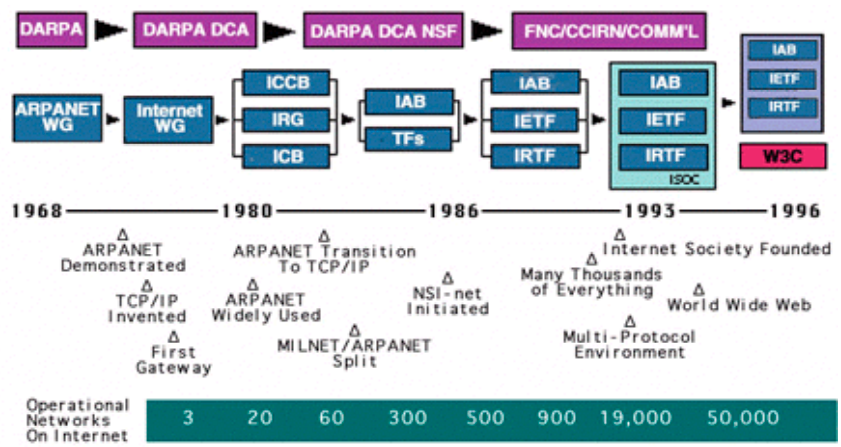
\includegraphics[width=15cm]{images/00/02}
\end{figure}

\Subsection{Стандартизирующие организации Internet}


Internet Society (ISOC)~--- сообщество, занимающееся развитием Internet
\begin{enumerate}
    \item Internet Architecture Board (IAB)~--- координирует развитие TCP/IP
    \begin{enumerate}
        \item Internet Engineering Steering Group (IESG)~--- рассмотрение стандартов и технические работы для IETF
        \item Internet Engineering Task Force (IETF)~--- самый главный комитет. Выпускают RFC
        \item Internet Research Task Force (IRTF)~--- развитие технологий, которые могут понадобиться в будущем
        \item Internet Corporation for Assigned Names and Numbers (ICANN)~--- централизованное назначение адресов и номеров (ранее IANA)
    \end{enumerate}
\end{enumerate}

\Subsection{Координирующие организации Internet}

Network Information Center (NIC)~--- организации, ответственные за распределение адресов
\begin{enumerate}
    \item InterNIC~--- США
    \item Reseaux IP Europeens (RIPE)~--- Европа
    \item African Network Information Centre (AfriNIC)~--- Африка
    \item Asia Pacific Network Information Centre (APNIC)~--- Азия
    \item Regional Latin-American and Caribbean IP Address Registry (LACNIC)~--- Латинская Америка
    \item Russian Institute for Public Networks (RIPN)~--- Россия
\end{enumerate}

\Subsection{Стандарты TCP/IP}

Все стандарты TCP/IP~--- это текстовые документы с уникальным номером (RFC). Все они лежат на ietf.org/rfc.html

Там нет жёсткой стандартизации, некоторые места можно истолковать двояко, не все им следуют.

Сначала их делили на FYI и STD. В последнее время так не делают

\Subsection{Иерархия протоколов TCP/IP}

\begin{figure}[H]
  \centering
  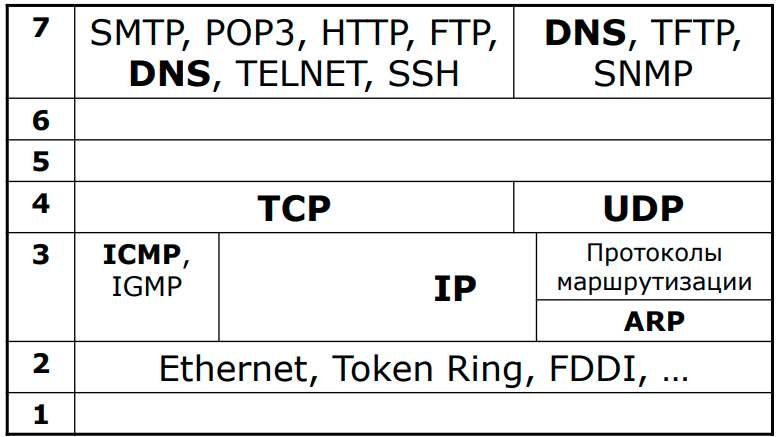
\includegraphics[width=15cm]{images/00/03}
\end{figure}

Самым важным протоколом является протокол сетевого уровня IP. На сетевом уровне находятся также ICMP (протокол управляющих сообщений, расширяет собой IP) и IGMP (протокол групповых сообщений), ARP (связь с канальным уровнем), огромное число протоколов маршрутизации.

На транспортном уровне TCP и UDP. 

На сеансовом уровне и уровне представления протоколов нет, поскольку кусок роли установления сеанса выполняет TCP (в UDP сеанса вообще нет). В TCP/IP шестого уровня нет. То есть каждый раз реализуем представительский протокол. Это жутко неудобно, привело к куче проблем и это архитектурная ошибка.

На прикладном уровне миллион разных протоколов. Слева транспорт TCP, справа~--- UDP. 


\Section{Адресация в IP}{Лекции 1-2}{Игорь Смирнов}

IP-адрес: 32 разряда

Записывается в виде десятичных октетов, разделённых точкой.

Можно адресовать $2^{32}$ узлов ($\approx 4\text{ млрд.}$)

Но не все из них поддерживаются.

Поддерживаются индивидуальная, групповая и широковещательная адресации.

Адресуется конкретный сетевой интерфейс, а не узел. Поэтому если у компьютера  сетевых интерфейса, то у него должно быть $\ge 3$ сетевых адреса. Некорректно говорить про IP-адрес узла.

И одному интерфейсу может соответствовать несколько IP-адресов. Например, если один интерфейс находится сразу в нескольких сетях.

Иногда (очень редко) можно дать один адрес нескольким интерфейсам.

Адресное пространство поделено на классы:

\begin{enumerate}
    \item Класс A~--- сети большого размера
    \item Класс B~--- сети среднего размера
    \item Класс C~--- небольшие сети
    \item Класс D~--- групповые адреса
    \item Класс E~--- для эКсПеРиМеНтОв
\end{enumerate}

Как это всё было изначально:

\Subsubsection{Адреса класса A}

Формат адреса: {\tt 0nnnnnnn.hhhhhhhh.hhhhhhhh.hhhhhhhh}

$n$~--- номер сети
$h$~--- номер узла

То есть можно сделать 128 сетей (а на самом деле 126, потому что 2 зарезервированы) по $2^{24}-2$ узлов в каждой.

Таким образом, все адреса в диапазоне {\tt 1.0.0.0-126.255.255.255}. Даже сейчас столько адресов ни одной компании не нужно. Поэтому их используют по-другому. Как именно~--- узнаем позже.

\Subsubsection{Адреса класса B}

Формат адреса: {\tt 10nnnnnn.nnnnnnnn.hhhhhhhh.hhhhhhhh}

{\tt n}~--- номер сети
{\tt h}~--- номер узла

$2^{14}$ сетей (тут уже нет двух зарезервированных), по $2^{16}-2$ узлов в каждой.

Диапазон адресов {\tt 128.0.0.0-191.255.255.255}

Это очень большие сети, таких размеров хватает крупнейшим корпорациям.

\Subsubsection{Адреса класса C}

Формат адреса: {\tt 110nnnnn.nnnnnnnn.nnnnnnnn.hhhhhhhh}

{\tt n}~--- номер сети
{\tt h}~--- номер узла

$2^{21}$ сетей, по 254 узла.

Диапазон адресов {\tt 192.0.0.0-223.255.255.255}

\Subsubsection{Адреса класса D}

Групповые адреса Internet.

Формат адреса: {\tt 1110xxxx.xxxxxxxx.xxxxxxxx.xxxxxxxx}

$2^{28}$ адресов, диапазон: {\tt 224.0.0.0 - 239.255.255.255}

Пример использования: вещание радиостанции на групповом адресе. Поднимаем на компьютере соответствующий IP-адрес. Тогда автоматически будет приходить нужный трафик.

К сожалению, используется редко (хотя зря).

\Subsubsection{Адреса класса E}

Зарезервированы для экспериментов

Формат адреса: {\tt 1111xxxx.xxxxxxxx.xxxxxxxx.xxxxxxxx}

$2^{28}$ адресов

Диапазон: {\tt 240.0.0.0-254.255.255.255}

Никогда пакет, приходящий из интернета не должен иметь класс E. Такие надо фильтровать.

\Subsection{Зарезервированные адреса}

\begin{MyItemize}
    \item Адрес {\tt 0.0.0.0}

    Если встречаете его в таблице маршрутизации, то это <<маршрут по умолчанию>>. Если встречаете его при адресации, то это <<данная сеть>>. Второе никогда не используется.
    \item Узел данной сети

    Вместо адреса сети записываем нули.

    A: {\tt 00000000.hhhhhhhh.hhhhhhhh.hhhhhhhh}\\
    B: {\tt 10000000.00000000.hhhhhhhh.hhhhhhhh}\\
    C: {\tt 11000000.00000000.00000000.hhhhhhhh}

    Но по факту это практически нигде не реализовано.

    \item Конкретная IP-сеть ($^*$)

    Вместо адреса узла~--- нули.

    A: {\tt 0nnnnnnn.00000000.00000000.00000000}\\
    B: {\tt 10nnnnnn.nnnnnnnn.00000000.00000000}\\
    C: {\tt 110nnnnn.nnnnnnnn.nnnnnnnn.00000000}

    Адресуем целую сеть. Используется в таблицах маршрутизации, когда хотим указать одинаковый маршрут для всей сети.

    \item Все узлы данной IP-сети ($^*$)

    Вместо адреса узла~--- единицы.

    A: {\tt 0nnnnnnn.11111111.11111111.11111111}\\
    B: {\tt 10nnnnnn.nnnnnnnn.11111111.11111111}\\
    C: {\tt 110nnnnn.nnnnnnnn.nnnnnnnn.11111111}

    Широковещательный адрес. Пакет придёт ко всем узлам этой сети. 

    Но по факту для сетей класса A и класса B не используется, потому что это мечта хакера. Посылаем 1 пакет, а его получают миллионы пользователей.

    Иногда блокируется вообще весь широковещательный трафик.

\end{MyItemize}

По сути последние два~--- это одно и то же. Только первое используется в таблицах маршрутизации, а второе в конкретных IP-пакетах, поэтому теоретически могли бы использовать только один из них, но почему-то так не сделали.

Из-за последних двух мы делали минус два, когда считали количество узлов в сети.

\begin{MyItemize}
    \item Все узлы данной локальной сети: {\tt 255.255.255.255}.

    Это отличается от <<Все узлы сети>> тем, что тут мы адресуем только те узлы, что подключены к нам канальным способом. То есть это широковещательный канальный адрес. В предыдущем же~--- сетевой уровень. Предыдущий маршрутизируется, а этот нет.

    \item Петля обратной связи.

    {\tt 01111111.xxxxxxxx.xxxxxxxx.xxxxxxxx}

    {\tt 127.0.0.1}~--- принято использовать.

    Не имеет внешнего выхода. Это обращение к самому себе через весь сетевой стек. 

    127~--- это сеть класса A. Нулевой и 127 занят, поэтому сетей класса A 126.
\end{MyItemize}

Так было в начале. Но потом добавили ещё несколько зарезервированных адресов.

IANA зарезервировала для внутреннего использования адреса <<неанонсированной сети>>. Когда разворачиваем локальную сеть и у нас нет полученных легальным образом адресов, мы можем использовать сеть из RFC1918:

\begin{MyItemize}
    \item {\tt 10.0.0.0-10.255.255.255}
    \item {\tt 172.16.0.0-172.31.255.255}
    \item {\tt 192.168.0.0-192.168.255.255}
\end{MyItemize}

Что будет если поставим себе другой адрес? Допустим, если мы поставили себе адрес майкрософта, мы отрежем себе доступ ко всему майкрософту.

А ещё есть зарезервированные адреса в сетях класса D.

\begin{MyItemize}
    \item {\tt 224.0.0.1}~--- все узлы данной подсети
    \item {\tt 224.0.0.2}~--- все маршрутизаторы данной подсети
    \item {\tt 224.0.0.5}~--- все OSPF маршрутизаторы
    \item {\tt 224.0.0.6}~--- все назначенные OSPF маршрутизаторы
    \item {\tt 224.0.0.9}~--- все RIP-2 маршрутизаторы
    \item {\tt 224.0.0.10}~--- все IGRP маршрутизаторы
\end{MyItemize}

\Subsection{Структуризация сетей IP}

В том, что мы обсуждали ранее много недостатков. Например, то, что много адресов вообще не используются. Поэтому придумали структуризацию сетей IP.

Теперь мы будем по-другому интерпретировать разряды адреса. Если раньше у нас были {\tt n} и {\tt h}, то теперь будет {\tt n}, {\tt s}, {\tt h}. {\tt s}~--- подсеть.

Маска подсети~--- это 32-х разрядный вектор флагов. Если в $i$-ом разряде маски стоит 1, то $i$-й разряд адреса содержит часть номера сети/подсети, а если 0, то часть номера узла.

Таким образом, с помощью адреса и маски, можно более гибко разделить сеть, чем с помощью адреса и класса.

Например, сеть класса C можем разделить на 2 подсети по 128 адресов с помощью маски {\tt 255.255.255.128}, на 4 подсети по 64 адреса с помощью маски {\tt 255.255.255.192}, 8 подсетей по 32 адреса с маской {\tt 255.255.255.224} ну и так далее.

Но вот 128 подсетей по 2 адреса~--- не работает. Потому что первый и последний адрес у нас зарезервированы. Поэтому минимальная подсеть содержит 4 адреса, 2 из которых зарезервированы.

Аналогично на подсети можно делить сети классов A и B.

В одной сети можно иметь подсети разного размера (стандарт VLSM).

Но у подсетей есть проблема (с первой и последней), потому что там есть широковещательные адреса (все нолики и все единички) и непонятно, к чему их применять (ко всей сети или к подсети). Поэтому сначала вообще не использовали первую и последнюю подсети. Однако потом подумали и поняли, что такая коллизия почти никогда не встречается, потому что всегда с нулевым адресом идёт маска, а широковещательную адресацию никто не использует. В итоге почти все маршрутизаторы позволяют использовать первую и последнюю подсети.

Принято, что сначала в маске идут разряды сети/подсети, а потом~--- узла (то есть префикс из единиц, а потом все нули). То есть теперь масок может быть всего 31 (маски из всех единиц быть не может, маска с одним ноликом бессмысленна). Кстати, маска с одной единицей тоже бессмысленна.

{\bf Префикс сети}~--- число единиц в маске (полагаем, что маска удовлетворяет предыдущему требованию).

Например, для маски {\tt 255.255.255.240} префикс сети~--- 28.

Подсеть записывается так: {\tt 195.19.212.96/27}, то есть IP-адрес первого узла, слеш и префикс. Этот адрес соответствует подсети {\tt 195.19.212.96-195.19.212.127}

Для стандартных сетей префиксы такие:
\begin{MyItemize}
    \item A~--- 8
    \item B~--- 16
    \item C~--- 24
\end{MyItemize}

\Subsubsection{Надсети}

Обратная идея: хотим объединять несколько соседних сетей.

Например, хотим объединить {\tt 195.19.212.0} и {\tt 195.19.213.0}

Объединим в надсеть {\tt 195.19.212.0/255.255.254.0} (префикс 23).

А теперь хотим объединить {\tt 192.168.1.0} и {\tt 192.168.2.0}.

Тут так не получится. Можем объединить только в сеть на 1024 адреса с префиксом 22: {\tt 192.168.0.0/255.255.252.0}

\Subsubsection{Задачки}

A~--- IP-адрес узла\\
M~--- маска подсети

Адрес подсети: {\tt Net = A\&M}\\
Широковещательный адрес: {\tt Broad=A|(!M)}\\
Размер подсети: {\tt K = (!M) - 1} (минус 1, потому что первый и последний адрес зарезервированы)

\Subsection{Адресация сервисов (приложений)}

{\bf Порт}~--- уникальный номер приложения на узле, использующего конкретный транспортный протокол.

В TCP/IP порт~--- это число от 0 до 65535.

Приложение в сети идентифицируется сокетом. {\bf Сокет}~--- это IP-адрес узла, тип транспортного протокола и номер порта.

Примеры:
\begin{MyItemize}
    \item TCP-сокет: {\tt 195.19.212.13:80}
    \item UDP-сокет: {\tt 195.19.212.10:53}
\end{MyItemize}

По соглашению, диапазон портов от 0 до 1023 зарезервирован за well-known серверными службами. Остальные, непривилегированные порты, могут использоваться любыми приложениями. 

\Section{Сетевой уровень TCP/IP}{Лекция 2}{Игорь Смирнов}

Протоколы:
\begin{itemize}
    \item IP~--- основной протокол архитектуры TCP/IP
    \item ICMP~--- протокол управляющих сообщений
    \item IGMP~--- протокол работы с группами
    \item ARP~--- протокол разрешения адресов~--- связь между собой адресов канального и сетевого уровней
    \item Протоколы маршрутизации
\end{itemize}

\Subsection{Протокол IP}

{\bf IP}~--- Internet Protocol

Стандарт RFC 791, 1981 год

Текущая действующая версия~--- 4 (IPv4)

Состоит из заголовка и тела

Суммарная длина до 64 Кбайт

Структура IP-пакета:

TODO: картинка

Ширина картинки~--- 32 разряда. Под каждым полем подписано, сколько разрядов оно занимает.

\begin{itemize}
    \item V~--- версия протокола
    \item HL~--- длина заголовка в 32-разрядных словах
    \item TOS~--- пожелания к процедуре обслуживания данного пакета
    \item Length~--- длина пакета в байтах
    \item ID~--- идентификатор (для фрагментации)
    \item F~--- флаги (для фрагментации)
    \item Offset~--- смещение (для фрагментации)
    \item TTL~--- время жизни
    \item Protocol~--- вложенный протокол (в данных)
    \item HCRC~--- контрольная сумма (по заголовку)
    \item Source Address~--- адрес отправителя
    \item Destination Address~--- адрес получателя
    \item Options~--- если пакет нестандартный и требует каких-то опций, можем их включить
    \item Pad~--- заполнитель, если опции не кратны 32 разрядам
    \item Data~--- данные
\end{itemize}

\Subsubsection{Поля заголовка пакета IP}

\begin{itemize}
    \item V~--- версия протокола (4)
    \item HL~--- длина заголовка в 32-разрядных словах (от 5 до 15). По дефолту 5, а эти 10 слов~--- на опции
    \item Length~--- длина пакета в байтах
    \item TTL~--- время жизни. Имело разный смысл. Изначально записывали значение <<время жизни пакета в секундах>> и маршрутизаторы отнимали из него время своей обработки. Сейчас это неактуально. Теперь каждый промежуточный маршрутизатор отнимает единицу. Если маршрутизатор получает 0, он удаляет пакет и посылает обратно ICMP сообщение. Время жизни нужно ограничивать, чтобы не зациклиться (мало ли где-то в сети есть петля маршрутизации). Утверждается, что между любыми узлами в сети интернет не более 29 промежуточных. То есть можно ставить 30.
    \item HCRC~--- контрольная сумма (по заголовку). Считается циклическим полиномом, по которому можно определить, не произошло ли искажения при передаче.
    \item Source Address~--- адрес отправителя
    \item Destination Address~--- адрес получателя
    \item Data~--- данные (тело пакета)
\end{itemize}

А где же записывается маска подсети? Она нужна только для процедуры маршрутизации, чтобы определить, каким путём посылать пакет. Самому пакету маски не нужны. 

\begin{itemize}
    \item Protocol~--- идентификатор вложенного протокола. Список идентификаторов лежит в RFC 1700. В операционных системах есть файл, который содержит код протокола ({\tt /etc/protocols}, {\tt \%systemroot\%$\backslash$system32$\backslash$drivers$\backslash$etc$\backslash$protocol})\\
    Основные протоколы:
    \begin{itemize}
        \item 1~--- ICMP
        \item 2~--- IGMP
        \item 4~--- IP4
        \item 6~--- TCP
        \item 17~--- UDP
        \item 89~--- OSPF
    \end{itemize}
    \item TOS~--- тип сервиса. Пожелания относительно способа доставки. В общем случае, пожелания могут быть проигнорированы. Но внутри своей сети можем запилить.\\
    TODO: картинка\\
    \begin{itemize}
        \item Приоритет (первые 3 разряда). Можно сделать очередь с приоритетом обработки пакетов (внутри своей сети).\\
        0~--- нормальный приоритет\\
        1~--- приоритетный\\
        2~--- немедленный\\
        3~--- мгновенный\\
        4~--- срочный\\
        5~--- критический\\
        6~--- межсетевое управление\\ 
        7~--- сетевое управление\\

        В жизни используются только 0, 1, 6, 7. Даже среди них 99\%~--- приоритет 0

        \item D (delay)~--- требуется минимальная задержка
        \item T (throughput)~--- требуется максимальная пропускная способность
        \item R (reliability)~--- требуется максимальная надёжность
        \item C (cost)~--- требуется минимальная стоимость
    \end{itemize}

    При этом одновременно может быть установлено 1 или 0 флагов.

    Для классических протоколов эти флаги предопределены.

    TODO: картинка.
\end{itemize}

\Subsubsection{Фрагментация пакетов} 

Напомним, что фрагментация поузловая.

\begin{itemize}
    \item Id~--- идентификатор, одинаковый у всех фрагментов. При передаче IP пакета это поле формируется псевдослучайно
    \item Offset~--- смещение фрагмента относительно начала пакета в 8-ми байтовых словах
    \item F~--- флаги
    \begin{itemize}
        \item 0~--- зарезервировано
        \item 1~--- флаг разрешения фрагментации. Если не установлен, маршрутизатор не имеет права фрагментировать данный пакет. А если она требуется, то пакет уничтожается, а обратно посылается ICMP пакет с ошибкой.
        \item 2~--- признак последнего фрагмента (внезапно, 0, если это последний фрагмент и 1 иначе)
    \end{itemize}

    Благодаря смещению правильно складываем куски в буффере, благодаря флагу последнего пакета понимаем, что все фрагменты пришли.

    На принимающей стороне есть таймер фрагментации, и если за это время все фрагменты не пришли, посылается ICMP сообщение.
\end{itemize}

\Subsubsection{Опции протокола IP}

Идёт прямо перед данными, может быть переменной длины. Может вообще не быть.

Это необязательные опции, используются только в служебных целях.

Формат опций:

TODO: картинка

\begin{itemize}
    \item Флаг копирования~--- 1, если нужно копировать опции во все фрагменты пакета. Если 0, то только в первом фрагменте
    \item Класс опции
    \begin{itemize}
        \item 0~--- управление дейтаграммами или сетью
        \item 1~--- зарезервировано
        \item 2~--- отладка сети
        \item 3~--- зарезервировано
    \end{itemize}
    \item Номер опции~--- номер внутри класса
\end{itemize}

Основные опции:

TODO: картинка
\begin{itemize}
    \item End of Option List~--- конец списка опций. Говорит, что это последняя опция в пакете. Нужна, если граница опций не совпадает с границей заголовка IP (когда есть паддинг). Занимает 1 байт.
    \item No operation~--- нет операции. Вспомогательная, для выравнивания границы опций, занимает 1 байт
    \item Stream ID~--- идентификатор потока. Например, хотим маршрутизировать видеотрафик. Всем пакетам одного потока присваивается одна метка потока. Понимаем, как маршрутизировать первый из них, а потом остальные маршрутизируем так же. Должна копироваться при фрагментации. Занимает 4 байта: 1 байт на заголовок, 1 байт на длину, 2 байта на идентификатор потока.
    \item Strict Source Route~--- строгая маршрутизация от источника (предопределённая маршрутизация). Пакет имеет право проходить только по адресам, указанным при отправке от источника и строго в указанном порядке.
    \begin{itemize}
        \item Заголовок
        \item Максимальная длина в байтах
        \item Указатель (на каком мы сейчас маршрутизаторе)~--- смещение в байтах от начала опции
        \item Список адресов.
    \end{itemize}
    Максимум можем указать 9 маршрутизаторов (так как есть ограницение на размер опций).
    \item Loose Source Route~--- нестрогая маршрутизация от источника. Содержит адреса маршрутизаторов, через которые должен пройти пакет. Формат такой же, как и раньше. Отличие в том, что мы снова обязаны пройти через все адреса, но при этом могут быть какие-то промежуточные.

    Обе эти опции использутся только для отладки.

    \item Record Route~--- запись маршрута. Используется в ping. В traceroute используется более хитрая схема.

    Есть несколько полей. Каждый маршрутизатор заполняет соответствующее ему поле своим адресом. Структура такая же как и у прошлых. Минус в том, что максимум 9 маршрутизатором сможем записать (опять из-за длины опций). Если все поля заняты, маршрутизатор просто ничего не делает.
\end{itemize}

{\bf Лирическое отступление: как работает traceroute?}

Отсылаем пакет с TTL=1, к нам обратно приходит ICMP пакет с ошибкой. Мы записываем адрес, с которого он пришёл, отправляем пакет с TTL=2 и так далее, пока не дойдём до конечного узла. Всё это время мы генерировали UDP пакет к случайному порту в старшем диапазоне. Как только он дошёл до конца, к нам пришлют ICMP пакет в котором будет сказано, что такой получатель недостижим. Так мы и поймём, что дошли до последнего узла.

Если за время посылок маршрут изменился, то мы получим неправильный маршрут в итоге.

Второй способ~--- использовать опцию Record Route. Но там максимум 9 промежуточных узлов. {\tt ping -r 9 -n 1 172.31.254.62}. Провайдер скорее всего фильтрует эту опцию, но в локальной сети использовать можно.

\Subsection{Связь с канальным уровнем}

Фрагментацию уже обсудили.

Нужно сопоставлять адреса. Например, IP-адреса и MAC-адреса. Для этого есть ARP-таблица. Одна строка в ней состоит из IP-адреса, MAC-адреса и типа записи. 

Типы записей:
\begin{enumerate}
    \item Динамические
    \item Статические
\end{enumerate}

Пусть каким-то чудом мы заполнили эту таблицу. Когда какой-то узел решает, что ему нужно свзаться с IP-адресом, который находится в нашей локальной сети (это можем узнать по маске и IP-адресу), ищем в ARP-таблице MAC-адрес, соответствующий данному IP-адресу. Если нашли, то радуемся. 

А вот если не нашли, то надо что-то придумывать.

ARP-таблица должна быть короткой, чтобы в ней был быстрый поиск, поэтому надо её как-то очищать от старой информации. 

Существует несколько политик очистки ARP-таблицы:
\begin{itemize}
    \item 10-минутное время жизни
    \item Время жизни записи 2 минуты, но при каждом новом обмене, время жизни обновляется
\end{itemize}

Есть утилита arp, с помощью которой можно посмотреть и поредактировать таблицу.

Как таблица заполняется? Статические записи вносятся ручками администратором. Это крайне редко и используется с какими-то редкими целями.

\Subsubsection{Протокол ARP}

Для динамического заполнения существует протокол ARP. Он один из самых старых, 1982 года. 

Для разных канальных сред есть разные RFC.

Кто-то хочет узнать адрес. Он посылает широковещательный запрос: <<У кого такой IP-адрес?>>. Ему отвечают (индивидуально): <<У меня такой IP-адрес!>>

Во время запроса и ответа заполняются {\it обе} ARP-таблицы.

Формат пакета ARP:

TODO: картинка

\begin{itemize}
    \item Network Type~--- тип протокола (для Ethernet~--- 1)
    \item Protocol~--- протокол сетевого уровня (IP~--- 2048)
    \item HAL~--- длина канального адреса (для MAC~--- 6 байт)
    \item PAL~--- длина сетевого адреса (для IP~--- 4 байта)
    \item Operation~--- тип операции (1~--- запрос, 2~--- ответ)
\end{itemize}

Этот протокол абсолютно незащищённый. Нет аутентификации. В открытом виде идёт запрос и в открытом виде идёт ответ. Можно просто обмануть и отправить ответ от своего имени. Хакер должен находиться в той же сети, что и жертва. 

Но при этом и запрашивающий компьютер получит два ответа, и второй узел увидит, что кто-то пытается использовать его адрес.

Поэтому хитрые хакеры на какое-то время выводят узел с запрашиваемым IP из строя.

Вариант защититься~--- всего один. Прописывать адреса ключевых узлов статически.

Эта атака нечастая, потому что хакер должен быть в вашей локальной сети.

А вот в старых виндах была проблема, что даже если вы прописали адрес маршрутизатора статически, то всё равно раз в минуту посылался ARP-запрос. В общем, не сидите в открытой сети с Windows 95.

Протокол ARP, так же как и IP, инкапсулируется прямо в канальный уровень.

\Subsubsection{Групповая доставка}

Раньше мы говорили об индивидуальной доставке. Но что если нам нужна групповая?

Во-первых, тогда нам (маршрутизатору) нужно будет знать о наличии групповых адресов в сегменте, чтобы не забивать канал групповыми сообщениями, если это не надо.

Во-вторых, машрутизатор должен периодически получать информацию о членстве в группах.

В третьих, нам нужен способ доставки групповых пакетов узлам. То есть нужно соответствие меду групповыми адресами сетевого и канального уровней.

Для индивидуальной адресации этим занимался протокол ARP, а для групповой это делается по-другому. 

В Ethernet адреса вида {\tt 01:xx:xx:xx:xx:xx} зарезервированы под групповые.

Конкретно под TCP/IP зарезервировали диапазон {\tt 01:00:5e:00:00:00-01:00:5e:7f:ff:ff}. Это 23 разряда.

Соостветствие между групповыми Ethernet и IP адреса~--- просто копирование младших 23 разрядов IP адреса в эти 23 разряда канального адреса.

Но в классе D было 28 разрядов, то есть мы игнорируем верхние 5 разрядов. В таком случае коллизии разрешаются уже на приёмной станции (если видим, что этот пакет не к нам~--- выкидываем).

А как маршрутизатор узнает, есть ли в сегменте групповы адреса? Для этого используется протокол {\bf IGMP}.

Весь следующий рассказ про {\bf IGMP v1}.

Он предназначен, чтобы информировать маршрутизатор о том, что в сегменте есть члены какой-то группы.

\begin{enumerate}
    \item Запрос: <<Есть ли подписчики такой-то группы в этом сегменте?>>
    \item Подписчики делают случайную задержу и посылают ответ: <<Да, есть!>>

    Случайная задержка нужна для того, чтобы если у нас есть 100500 подписчиков в сегменте, то один из них (с минимальной задержкой) отошлёт ответ, остальные это увидят и свой ответ посылать не будут (маршрутизатору важно знать, что хоть кто-то там есть).
    \item Если на какой-то запрос не пришёл ответ (через таймаут), то маршрутизатор считает, что подписчиков этой группы нет.
\end{enumerate}

Формат пакета IGMP v1:

TODO: картинка.

\begin{itemize}
    \item Тип~--- запрос (1) или ответ (2)
    \item Адрес группы~--- в запросе~--- 0, в ответе~--- номер группы, о которой мы нотифицируем маршрутизатор <<Эта группа есть в данном сегменте>>
\end{itemize}

Протокол IGMP инкапсулируется в протокол IP. В IP-пакете используется:
\begin{itemize}
    \item Адрес {\tt 224.0.0.1}
    \item TTL=1 (чтобы не маршрутизировался)
\end{itemize}

IGMP v2 обратно совместим с v1.

TODO: картинка

Поле <<Тип>> занимает 1 байт.
\begin{itemize}
    \item {\tt 0x11}~--- запрос о членстве в группах или конкретной группе
    \item {\tt 0x16}~--- отчёт о членстве v2
    \item {\tt 0x17}~--- нотификация о покидании группы
    \item {\tt 0x12}~--- отчёт о членстве v1 (для совместимости)
\end{itemize}

Максимальное время ответа в 0.1 секунды.

IGMP v3 обратно совместим с v1 и v2.

Позволяет запросить несколько групп и отчитаться о членстве в нескольких группах.

Все версии протокола IGMP не шифруются (а значит, такие же слабости, как и у ARP).

Протокол IP тоже не шифруется, у него нет никаких средств защиты, кроме контрольной суммы, которая тоже такое себе средство защиты. Поэтому вся защита сделана на более высоких уровнях.

\end{document}
